% Figure from MATH 591 notes, section 2. Compile with the notes preamble.
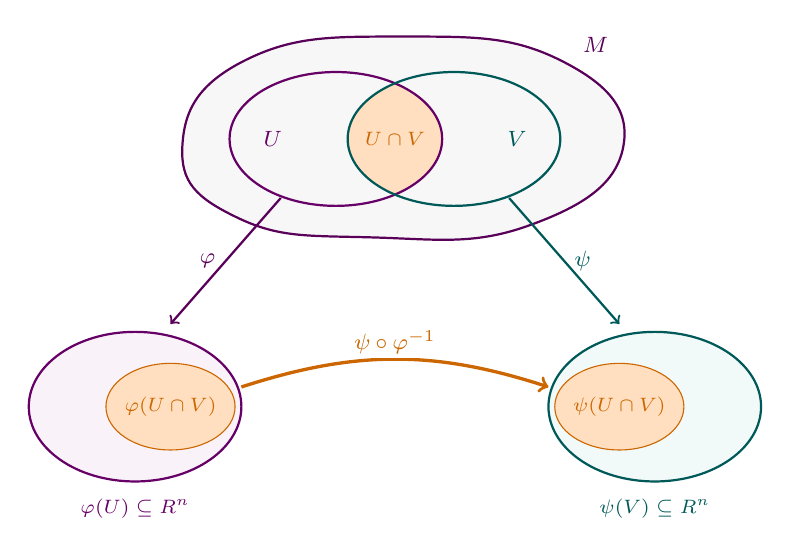
\begin{tikzpicture}
\draw[thick, violet!70!black, fill=gray!6] plot[smooth cycle, tension=0.8] coordinates {(-2.7,3.0) (-1.9,4.1) (0.1,4.4) (2.1,4.1) (2.9,3.0) (1.7,2.0) (-0.3,1.85) (-2.0,2.1)};
\begin{scope} \clip (-0.75,3.1) ellipse (1.35 and 0.85); \fill[orange!25] (0.75,3.1) ellipse (1.35 and 0.85); \end{scope}
\draw[violet!80!black, thick] (-0.75,3.1) ellipse (1.35 and 0.85); \draw[teal!70!black, thick] (0.75,3.1) ellipse (1.35 and 0.85);
\node[violet!80!black, font=\footnotesize] at (-1.55,3.1) {$U$}; \node[teal!70!black, font=\footnotesize] at (1.55,3.1) {$V$}; \node[orange!80!black, font=\scriptsize] at (0,3.1) {$U\cap V$};
\node[violet!70!black, font=\footnotesize] at (2.55,4.3) {$M$};
\draw[violet!80!black, thick, fill=violet!5] (-3.3,-0.3) ellipse (1.35 and 0.95); \fill[orange!25] (-2.85,-0.3) ellipse (0.82 and 0.55); \draw[orange!80!black] (-2.85,-0.3) ellipse (0.82 and 0.55);
\draw[teal!70!black, thick, fill=teal!5] (3.3,-0.3) ellipse (1.35 and 0.95); \fill[orange!25] (2.85,-0.3) ellipse (0.82 and 0.55); \draw[orange!80!black] (2.85,-0.3) ellipse (0.82 and 0.55);
\node[violet!80!black, font=\scriptsize, align=center] at (-3.3,-1.6) {$\varphi(U) \subseteq \mathbb{R}^n$}; \node[teal!70!black, font=\scriptsize, align=center] at (3.3,-1.6) {$\psi(V) \subseteq \mathbb{R}^n$};
\node[orange!80!black, font=\scriptsize] at (-2.85,-0.3) {$\varphi(U\cap V)$}; \node[orange!80!black, font=\scriptsize] at (2.85,-0.3) {$\psi(U\cap V)$};
\draw[->, thick, violet!70!black] (-1.45,2.35) -- node[left, font=\footnotesize] {$\varphi$} (-2.85,0.75);
\draw[->, thick, teal!70!black] (1.45,2.35) -- node[right, font=\footnotesize] {$\psi$} (2.85,0.75);
\draw[->, very thick, orange!80!black] (-1.95,-0.05) to[bend left=18] node[above, font=\footnotesize, fill=white, inner sep=1.5pt] {$\psi\circ\varphi^{-1}$} (1.95,-0.05);
\end{tikzpicture}
